\chapter{Design and Implementation}


The main goal of this thesis is to be able to recognize asbestos fibers in microscopic images. To achieve that goal different CNN architectures are evaluated and altered to better meet this specific problems' characteristics. Different methods like transfer learning and data augmentation are applied to this problem in hope to further increase the accuracy. This is especially important, since the provided dataset consists of only a few hundred images to learn from. There is no baseline available, so a new baseline needs to be established with a simple CNN.

\section{Problem Description}

The provided dataset consists of about 2'000 microscopic images with and without asbestos fibers. The images come in two different dimensions and different qualities. Most of the images are 1024 by 768 pixels but some are in 1024 by 1024 pixels. Only a small subset was pre-labled and the remaining images needed to be labeled by hand, an error-prone task since I was never professionally instructed on how to do it. After labeling the images, they were send back to the laboratories for checking, but there were many images, that the experts were uncertain on how to label them. From 441 images I labeled and send the laboratory for checking 78 images came back as being suspected to contain asbestos but they were not quite sure. That's about 5.65\%. The detection of traces of asbestos by images is indeed very difficult and the error rate increases significantly as stated by the laboratory. In Figure \ref{fig:basic_examples} three example images are shown. One with asbestos, one without and one image with an error, that makes it difficult to be used for the training.

\begin{figure}[t]
\centering
\subfigure[Example with an asbestos fiber spanning from top to down]{
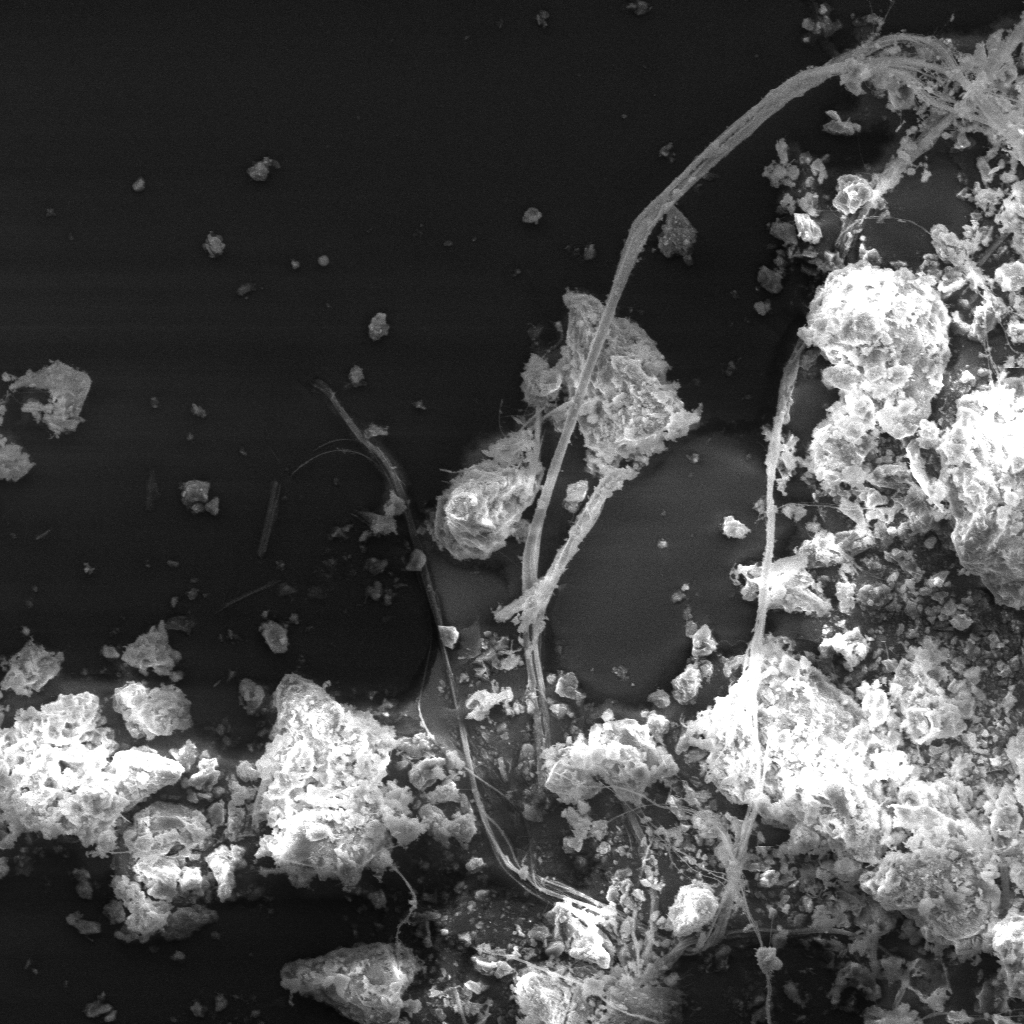
\includegraphics[width=.3\textwidth]{images/chapter4/asbestos.png}
}
\subfigure[Example without any asbestos fibers]{
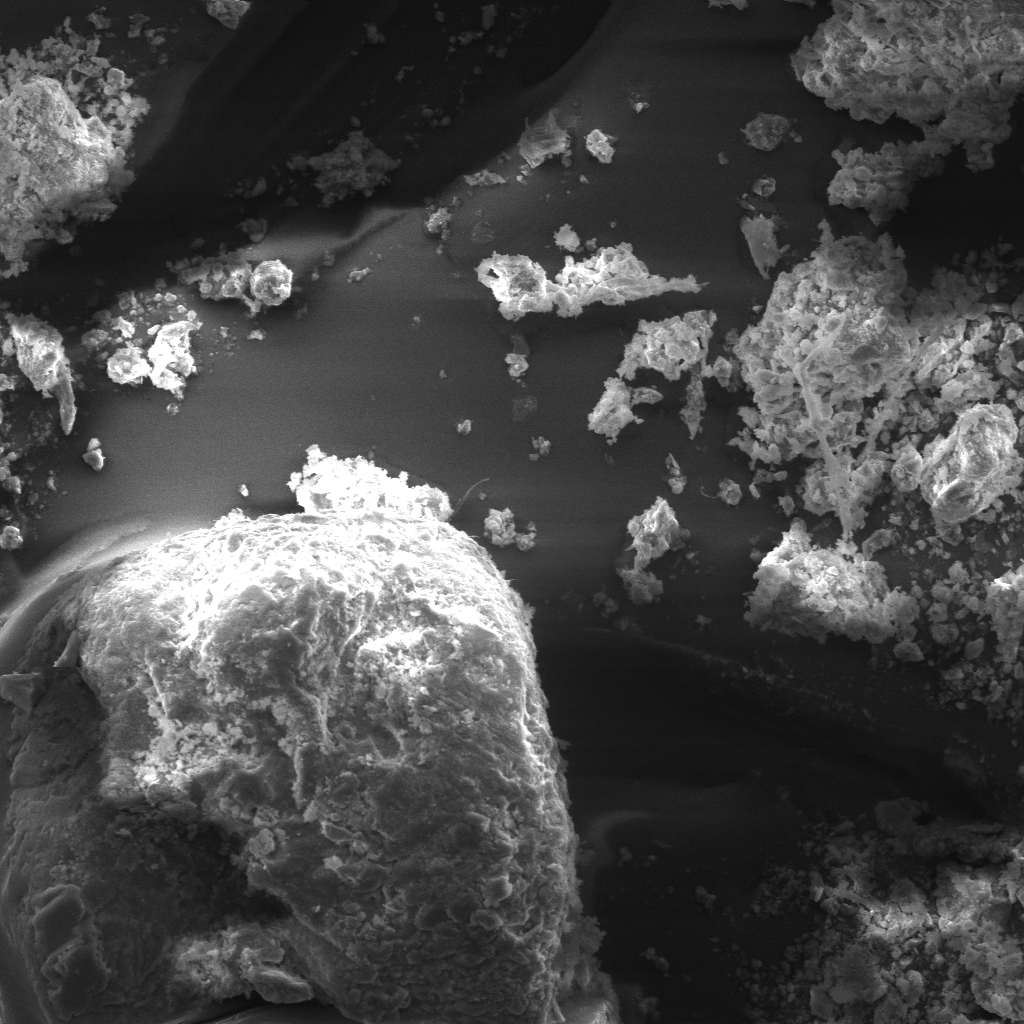
\includegraphics[width=.3\textwidth]{images/chapter4/non-asbestos.png}
}
\subfigure[Example of one kind of error, that makes the image unusable]{
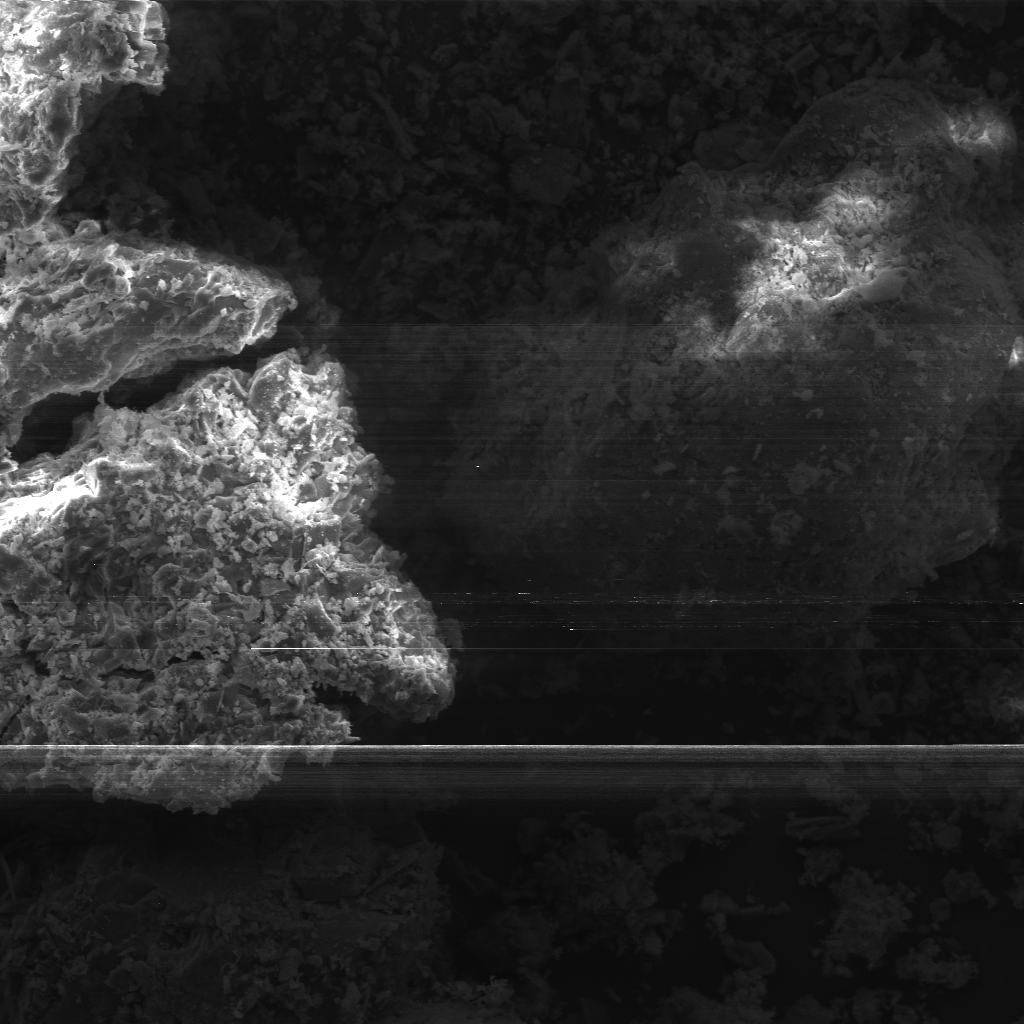
\includegraphics[width=.3\textwidth]{images/chapter4/fail.png}
}
\caption{Some examples on how the microscopic images look like, and what kind of error in images occur.}
\label{fig:basic_examples}
\end{figure}

Since the images are quite large, they will drastically increase in size, once decoded into a PIL object, or Tensor object. Therefore it will be difficult to train on the whole image due to GPU resource restrictions. For the project, four Tesla K80 with 12GB of RAM each were provided.

[**I think the 0.1\% they mention holds true only for clear cases where there is lots of asbestos.**]

\section{Dataset}

There are two valid datasets that were manually labeled and partially verified. The bigger dataset has more labels that are less clear and suspected to have or have not asbestos in them. Images with minor errors, as shown above, are not removed from the training and validation sets. In the smaller datasets, I removed all the images, that were unclear to me. I also removed the images with errors in them.

[[ do I need to provide two links to the datasets? I could link them to my dropbox account ]]


\section{Data Augmentation}

One common problem in Deep Learning is the amount of data needed to be able to train a model well. This requirement of having huge datasets arises from the need to train a large number of parameters of the model, which usually goes into the millions for current state-of-the-art architecuters like VGG's \cite{simonyan2014very}, ResNet's \cite{he2016deep} or Inception [TODO: ref]. Tuning these parameters leads to a lower loss and hopefully to a higher generalizability. Having not enough images to train on will lead to poor inference from the data that overfits to the current images and not generalize well to a unseen test-set. Many studies have found a correlation between overall performance of the model and its size (number of parameters and layers) with lower layers of the model capturing very basic information like horizontal and vertical lines or color gradients and higher layers capturing the overall structure of the object that takes in more of the spatial characteristics. [TODO: Maybe my task is not simple but it requires much less parameters since it is only a binary classification and asbestos is not that complex to recognize]

There are only a few hundred good and usable images provided for the asbestos recognition task. Additionally they are highly specialized in how they were done. With specific cameras and in specific environments in a specific zoom. Finding more images on the internet is impossible so data augmentation could possibly lead to an increased dataset with more images to train on and therefore increase performance. A huge dataset is required to be able to generalize the model and to perform well on a test set. Transfer learning might help but the fine tuning needs to be done after transferring the weights to the current task.

There two main forms of data augmentation. Offline and online augmentation. With offline data augmentation the images are augmented seperately and saved to disk. This increases the overall size of the dataset by as many transformations that are done on an image. E.g. flipping horizontally and vertically would result in a three time increase of the dataset. The convolutional neural network would be able to more robustly classify objects in different places and different orientations leading to increased invariance. The downside of offline augmentation is the incrase of disk space and therfore disk I/O during training that slows down the learning, and that it results in a very static training process. Adding more epochs would mean to learn more time on the same set of images present on disk.
Online data augmentation happens on the fly and does not need more disk space and disk I/O since it all happens in memory. The image is first loaded into memory and then several transformations are applied to the image. These transformations can be flipping, rotating, scaling, distorting and cropping in different places, and it all can be done randomly. Especially the rotating and cropping when done randomly yields new images with every new epoch. Online augmentation is therefore preferred since it leads to faster learning while reducing overfitting to the current images.

\section{Transfer Learning}

Finding millions of images on the internet of day-to-day objects is an easy task. Finding images on specialized objects like cancer cells in certain tissues is almost impossible. Especially when the equipment with all the settings is also different from hospital to hospital. To mitigate this problem transfer learning can be applied. With this method, the pre-learned weights for a certain architecture can be downloaded from the internet. These weights were obtained learning the model for a long time (until convergence) with a dataset like ImageNet. The hope is that the lower layer features are very similar even across problem domains. E.g. the cancer tumor has edges and colors like any real world object from the ImageNet dataset. These can be used and fine-tuned. This gives the model a much better starting point other than initializing all weights of the model randomly and training them from scratch.

It has been shown that pre-training on ImageNet indeed yields better results through obtaining good general-purpose features in tasks like image classification \cite{sharif2014cnn} and object detection \cite{girshick2014rich, sermanet2013overfeat} But when the target domain is even farther away like for example human pose estimation \cite{carreira2016human}, image segmentation \cite{dai2016instance} and image captioning \cite{donahue2015long, karpathy2015deep}, pre-training on ImageNet may help. Transfer learning has become the de facto standard for solving a many different computer vision problems because it promises faster convergence and better accuracies despite the datasets getting bigger and the architectures deeper \cite{huh2016makes}. Applying transfer learning therefore speeds up the process of finding and developing good architectures.

This common knowledge that transfer learning always helps even across different target domains is not without critic. He et al. chanllenge this approach in a paper published in 2018 \cite{he2018rethinking}. They couldn't show that pre-training yielded better results on the COCO dataset than random initialization (training from scratch), only that it speeds up convergence very early in training. Better regularization and final target task accuracies were not obtained with pre-training. The main benefit of pre-training is that it converges faster and therefore training from scratch takes longer to catch up.

\section{AlexNext}

It has not been possible to get a baseline for the current performance or even an accurate estimation of human performance in the detection of asbestos fibers in the provided images. Therefore, AlexNet was used to create a baseline on which improvements may be observed and would allow discussions on architectures and their performance. The hyper-parameters learning rate and learning rate decay have been optimized with grid search as shown in Table \ref{tbl:similarity-test-map}. The model has been run for 50 epochs, although convergence has been observed much earlier as seen in Figure XXX.

\begin{table}[t] \centering
\ra{1.3}
\caption{AlexNet accuracies for baseline with optimized hyper-parameters}
\begin{tabular}{@{}rrrr@{}}
\toprule & learning rate & lr-decay & accuracy \\
\midrule
AlexNet		& 0.1 		& 5		& 52.18\%  \\
AlexNet		& 0.05 		& 5		& 53.64\%  \\
AlexNet		& 0.01 		& 5		& 53.37\%  \\
AlexNet		& 0.005 		& 5		& 53.67\%  \\
AlexNet		& 0.001 		& 5		& 78.82\%  \\
AlexNet		& 0.0005 		& 5		& 78.55\%  \\
AlexNet		& 0.0001 		& 5		& 77.09\%  \\
\bottomrule
\end{tabular}
\label{tbl:AlexNetBaseline}
\end{table}


\section{Inception / ResNet}

Talk about other architectures and why they are important

\section{SigOpt Optimization}

What is SigOpt and why did I use it?

\section{ResNet18 alterations}

Talk extensively about my new architectures where I try increase the input image. I actually achieved best results with the old dataset of around 93\% accuracy with going down with the filters.... so from some million parameters I went  down to only 40'000 parameters and achieved best results... I will have to go into this much more

\section{Visualization}

Talk about different visualizations and what kind of visualizations make sense for this problem, what can be deduced from it and so on... 